\subsection{Sub\-Image  Class Reference}
\label{class_subimage}\index{SubImage@{Sub\-Image}}
a class that allows to cut a subimage from a {\bf Reduced\-Image} {\rm (p.\,\pageref{class_reducedimage})}. 


{\tt \#include $<$subimage.h$>$}

Inheritance diagram for Sub\-Image::\begin{figure}[H]
\begin{center}
\leavevmode
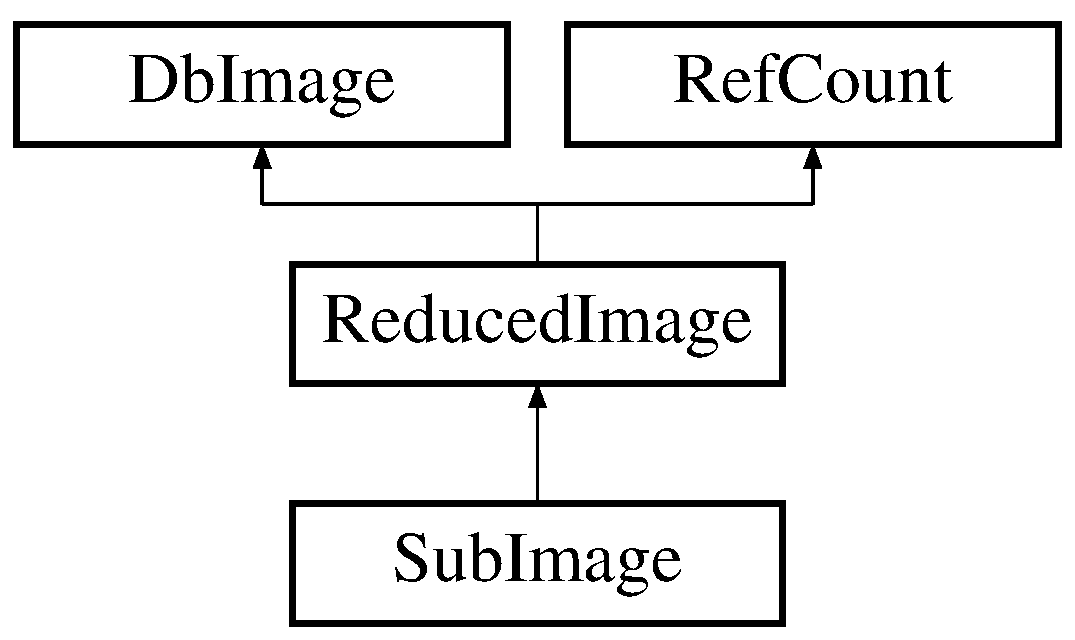
\includegraphics[height=3cm]{class_subimage}
\end{center}
\end{figure}
\subsubsection*{Public Methods}
\begin{CompactItemize}
\item 
\index{SubImage@{SubImage}!SubImage@{Sub\-Image}}\index{SubImage@{SubImage}!SubImage@{Sub\-Image}}
{\bf Sub\-Image} ()\label{class_subimage_a0}

\item 
\index{SubImage@{SubImage}!SubImage@{Sub\-Image}}\index{SubImage@{SubImage}!SubImage@{Sub\-Image}}
{\bf Sub\-Image} (const string \&Name, const string \&Large\-Image\-Name, const {\bf Frame} \&Sub\-Frame)\label{class_subimage_a1}

\item 
\index{MakeFits@{MakeFits}!SubImage@{Sub\-Image}}\index{SubImage@{SubImage}!MakeFits@{Make\-Fits}}
bool {\bf Make\-Fits} ()\label{class_subimage_a2}

\begin{CompactList}\small\item\em produce fits image.\item\end{CompactList}\item 
\index{MakeWeight@{MakeWeight}!SubImage@{Sub\-Image}}\index{SubImage@{SubImage}!MakeWeight@{Make\-Weight}}
bool {\bf Make\-Weight} ()\label{class_subimage_a3}

\item 
\index{MakeCosmic@{MakeCosmic}!SubImage@{Sub\-Image}}\index{SubImage@{SubImage}!MakeCosmic@{Make\-Cosmic}}
bool {\bf Make\-Cosmic} ()\label{class_subimage_a4}

\begin{CompactList}\small\item\em produce cosmic image.\item\end{CompactList}\item 
\index{MakeSatellite@{MakeSatellite}!SubImage@{Sub\-Image}}\index{SubImage@{SubImage}!MakeSatellite@{Make\-Satellite}}
bool {\bf Make\-Satellite} ()\label{class_subimage_a5}

\begin{CompactList}\small\item\em produce satellite image.\item\end{CompactList}\item 
\index{MakeSatur@{MakeSatur}!SubImage@{Sub\-Image}}\index{SubImage@{SubImage}!MakeSatur@{Make\-Satur}}
bool {\bf Make\-Satur} ()\label{class_subimage_a6}

\begin{CompactList}\small\item\em produce satur image.\item\end{CompactList}\item 
\index{MakeDead@{MakeDead}!SubImage@{Sub\-Image}}\index{SubImage@{SubImage}!MakeDead@{Make\-Dead}}
bool {\bf Make\-Dead} ()\label{class_subimage_a7}

\begin{CompactList}\small\item\em produce dead image.\item\end{CompactList}\item 
\index{MakeCatalog@{MakeCatalog}!SubImage@{Sub\-Image}}\index{SubImage@{SubImage}!MakeCatalog@{Make\-Catalog}}
bool {\bf Make\-Catalog} ()\label{class_subimage_a8}

\begin{CompactList}\small\item\em Produce the Saturated stars pixels mask, subtract the image background, detect with the SExtractor computed sigma. search the cosmics, and update catalog and weight for cosmics. No free coffee.\item\end{CompactList}\item 
\index{Clone@{Clone}!SubImage@{Sub\-Image}}\index{SubImage@{SubImage}!Clone@{Clone}}
{\bf Reduced\-Image}$\ast$ {\bf Clone} () const\label{class_subimage_a9}

\end{CompactItemize}


\subsubsection{Detailed Description}
a class that allows to cut a subimage from a {\bf Reduced\-Image} {\rm (p.\,\pageref{class_reducedimage})}.



The documentation for this class was generated from the following file:\begin{CompactItemize}
\item 
{\bf subimage.h}\end{CompactItemize}
